\documentclass[11pt,a4paper]{article}

% ============================================
% PACKAGES
% ============================================
\usepackage[utf8]{inputenc}
\usepackage[T1]{fontenc}
\usepackage{lmodern}
\usepackage[margin=0.9in]{geometry}
\usepackage{hyperref}
\usepackage{xcolor}
\usepackage{listings}
\usepackage{tcolorbox}
\usepackage{booktabs}
\usepackage{longtable}
\usepackage{tabularx}
\usepackage{array}
\usepackage{enumitem}
\usepackage{titlesec}
\usepackage{fancyhdr}
\usepackage{graphicx}
\usepackage{tikz}
\usepackage{parskip}
\usetikzlibrary{shapes.geometric, arrows, positioning, fit, backgrounds}

% ============================================
% COLORS
% ============================================
\definecolor{codegreen}{rgb}{0,0.6,0}
\definecolor{codegray}{rgb}{0.5,0.5,0.5}
\definecolor{codepurple}{rgb}{0.58,0,0.82}
\definecolor{backcolour}{rgb}{0.95,0.95,0.92}
\definecolor{accentblue}{RGB}{0, 102, 204}
\definecolor{accentgreen}{RGB}{0, 153, 76}
\definecolor{warningorange}{RGB}{255, 153, 0}
\definecolor{importantred}{RGB}{204, 0, 0}

% ============================================
% CODE LISTING STYLE
% ============================================
\lstdefinestyle{pythonstyle}{
    backgroundcolor=\color{backcolour},
    commentstyle=\color{codegreen},
    keywordstyle=\color{accentblue}\bfseries,
    numberstyle=\tiny\color{codegray},
    stringstyle=\color{codepurple},
    basicstyle=\ttfamily\footnotesize,
    breakatwhitespace=false,
    breaklines=true,
    captionpos=b,
    keepspaces=true,
    numbers=left,
    numbersep=5pt,
    showspaces=false,
    showstringspaces=false,
    showtabs=false,
    tabsize=4,
    language=Python,
    frame=single,
    rulecolor=\color{codegray}
}
\lstset{style=pythonstyle}

% ============================================
% TCOLORBOX STYLES
% ============================================
\tcbuselibrary{skins,breakable}

\newtcolorbox{importantbox}{
    colback=importantred!5!white,
    colframe=importantred!75!black,
    fonttitle=\bfseries,
    title=Important,
    breakable
}

\newtcolorbox{notebox}{
    colback=accentblue!5!white,
    colframe=accentblue!75!black,
    fonttitle=\bfseries,
    title=Note,
    breakable
}

\newtcolorbox{tipbox}{
    colback=accentgreen!5!white,
    colframe=accentgreen!75!black,
    fonttitle=\bfseries,
    title=Tip,
    breakable
}

\newtcolorbox{qabox}[1]{
    colback=warningorange!5!white,
    colframe=warningorange!75!black,
    fonttitle=\bfseries,
    title=Q: #1,
    breakable
}

\newtcolorbox{decisionbox}[1]{
    colback=accentgreen!5!white,
    colframe=accentgreen!75!black,
    fonttitle=\bfseries,
    title=Decision: #1,
    breakable
}

% ============================================
% HEADER/FOOTER
% ============================================
\pagestyle{fancy}
\fancyhf{}
\rhead{Iris Backend Architecture Guide}
\lhead{\leftmark}
\rfoot{Page \thepage}
\renewcommand{\headrulewidth}{0.4pt}
\renewcommand{\footrulewidth}{0.4pt}

% ============================================
% TITLE FORMATTING
% ============================================
\titleformat{\section}
    {\Large\bfseries\color{accentblue}}
    {\thesection}{1em}{}
\titleformat{\subsection}
    {\large\bfseries\color{accentblue!80!black}}
    {\thesubsection}{1em}{}
\titleformat{\subsubsection}
    {\normalsize\bfseries\color{accentblue!60!black}}
    {\thesubsubsection}{1em}{}

% ============================================
% HYPERREF SETUP
% ============================================
\hypersetup{
    colorlinks=true,
    linkcolor=accentblue,
    filecolor=magenta,
    urlcolor=accentblue,
    pdftitle={Iris Backend Architecture Guide},
    pdfauthor={Developer},
    bookmarks=true
}

% ============================================
% DOCUMENT
% ============================================
\begin{document}

% ============================================
% TITLE PAGE
% ============================================
\begin{titlepage}
    \centering
    \vspace*{2cm}
    
    {\Huge\bfseries\color{accentblue} Iris Backend\\[0.3cm] Architecture Guide}
    
    \vspace{1cm}
    
    {\Large Wikipedia Pathfinding Engine}
    
    \vspace{2cm}
    
    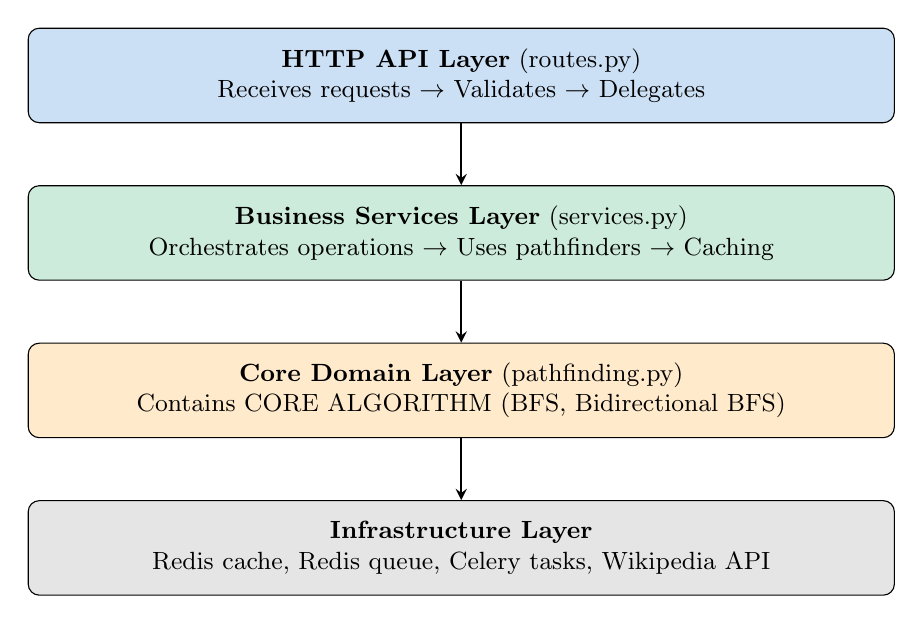
\begin{tikzpicture}[
        layer/.style={draw, rounded corners, minimum width=11cm, minimum height=1.2cm, align=center, font=\small},
        arrow/.style={->, thick, >=stealth}
    ]
        \node[layer, fill=accentblue!20] (api) at (0,4) {\textbf{HTTP API Layer} (routes.py)\\Receives requests $\rightarrow$ Validates $\rightarrow$ Delegates};
        \node[layer, fill=accentgreen!20] (services) at (0,2) {\textbf{Business Services Layer} (services.py)\\Orchestrates operations $\rightarrow$ Uses pathfinders $\rightarrow$ Caching};
        \node[layer, fill=warningorange!20] (core) at (0,0) {\textbf{Core Domain Layer} (pathfinding.py)\\Contains CORE ALGORITHM (BFS, Bidirectional BFS)};
        \node[layer, fill=codegray!20] (infra) at (0,-2) {\textbf{Infrastructure Layer}\\Redis cache, Redis queue, Celery tasks, Wikipedia API};
        
        \draw[arrow] (api) -- (services);
        \draw[arrow] (services) -- (core);
        \draw[arrow] (core) -- (infra);
    \end{tikzpicture}
    
    \vspace{2cm}
    
    {\large Interview Preparation \& Development Reference}
    
    \vfill
    
    {\large Last Updated: January 2026}
\end{titlepage}

% ============================================
% TABLE OF CONTENTS
% ============================================
\tableofcontents
\newpage

% ============================================
% SECTION 1: PROJECT STRUCTURE
% ============================================
\section{Project Structure Overview}

The Iris backend follows a \textbf{Clean Architecture} pattern with clear separation of concerns.

\begin{lstlisting}[language=bash, style=pythonstyle, caption=Project Directory Structure]
iris-web-backend/
|-- app/                          # Main application package
|   |-- __init__.py              # Flask app factory & Celery setup
|   |-- api/                     # HTTP API layer
|   |   |-- routes.py            # API endpoints (Flask blueprints)
|   |   |-- middleware.py        # Decorators: error handling, logging, CORS
|   |   |-- schemas.py           # Marshmallow schemas for validation
|   |-- core/                    # Core business logic (THE BRAIN)
|   |   |-- factory.py           # Dependency Injection (ServiceFactory)
|   |   |-- interfaces.py        # Abstract interfaces (contracts)
|   |   |-- models.py            # Data models (dataclasses)
|   |   |-- pathfinding.py       # CORE ALGORITHM (BFS)
|   |   |-- services.py          # Business services orchestration
|   |-- external/                # External API integrations
|   |   |-- wikipedia.py         # Wikipedia API client
|   |-- infrastructure/          # Infrastructure concerns
|   |   |-- cache.py             # Redis cache implementation
|   |   |-- redis_queue.py       # Redis queue for BFS state
|   |   |-- tasks.py             # Celery background tasks
|   |-- utils/                   # Utilities
|       |-- exceptions.py        # Custom exception hierarchy
|       |-- logging.py           # Logging configuration
|-- config/                      # Configuration classes
|-- tests/                       # Test suites
|-- run.py                       # Application entry point
|-- celery_worker.py             # Celery worker entry point
\end{lstlisting}

% ============================================
% SECTION 2: ARCHITECTURE LAYERS
% ============================================
\section{Architecture Layers}

The codebase follows a \textbf{layered architecture} similar to Clean Architecture. Each layer has a single responsibility.

\subsection{Layer Descriptions}

\begin{tabularx}{\textwidth}{@{}>{\bfseries}l X@{}}
\toprule
Layer & Responsibility \\
\midrule
HTTP API Layer \newline \footnotesize\texttt{app/api/} & 
Receives HTTP requests, validates input using Marshmallow schemas, applies cross-cutting middleware (CORS, logging, error handling), delegates to business services, and formats JSON responses. \\
\addlinespace[0.5em]
Business Services \newline \footnotesize\texttt{app/core/services.py} & 
Orchestrates business operations. Checks cache before invoking pathfinding, coordinates between pathfinders and Wikipedia client, encapsulates use cases like ``find path'' or ``explore page.'' \\
\addlinespace[0.5em]
Core Domain \newline \footnotesize\texttt{app/core/pathfinding.py} & 
Contains the pure BFS algorithm. No knowledge of HTTP, Redis, or Flask. Only knows about abstract interfaces. This is where the graph traversal logic lives. \\
\addlinespace[0.5em]
Infrastructure \newline \footnotesize\texttt{app/infrastructure/} & 
Concrete implementations: Redis cache, Redis queue for BFS state, Celery tasks for background processing, Wikipedia API client. All ``how'' details live here. \\
\bottomrule
\end{tabularx}

\subsection{Data Flow Diagram}

\begin{center}
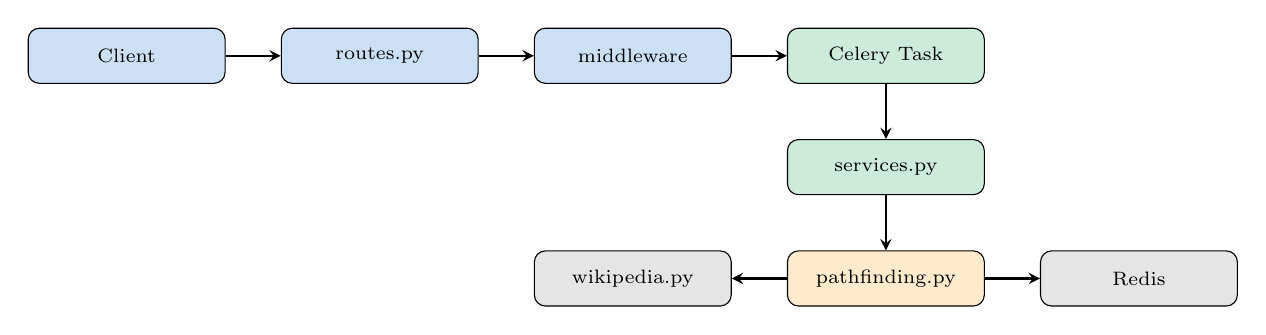
\begin{tikzpicture}[
    node distance=0.7cm,
    box/.style={draw, rounded corners, minimum width=2.5cm, minimum height=0.7cm, align=center, font=\scriptsize},
    arrow/.style={->, thick, >=stealth}
]
    \node[box, fill=accentblue!20] (client) {Client};
    \node[box, fill=accentblue!20, right=of client] (routes) {routes.py};
    \node[box, fill=accentblue!20, right=of routes] (middleware) {middleware};
    \node[box, fill=accentgreen!20, right=of middleware] (celery) {Celery Task};
    \node[box, fill=accentgreen!20, below=of celery] (services) {services.py};
    \node[box, fill=warningorange!20, below=of services] (pathfinding) {pathfinding.py};
    \node[box, fill=codegray!20, left=of pathfinding] (wikipedia) {wikipedia.py};
    \node[box, fill=codegray!20, right=of pathfinding] (redis) {Redis};
    
    \draw[arrow] (client) -- (routes);
    \draw[arrow] (routes) -- (middleware);
    \draw[arrow] (middleware) -- (celery);
    \draw[arrow] (celery) -- (services);
    \draw[arrow] (services) -- (pathfinding);
    \draw[arrow] (pathfinding) -- (wikipedia);
    \draw[arrow] (pathfinding) -- (redis);
\end{tikzpicture}
\end{center}

% ============================================
% SECTION 3: ARCHITECTURE DECISIONS
% ============================================
\section{Architecture Decisions \& Engineering Rationale}

This section justifies key technical decisions from a \textbf{distributed systems} and \textbf{scalability} perspective. These are the answers that demonstrate engineering depth.

\subsection{High-Level Architecture Decisions}

\begin{decisionbox}{Asynchronous Task Processing with Celery}
\textbf{Problem:} Wikipedia pathfinding can take 30 seconds to 5+ minutes. HTTP requests would timeout.

\textbf{Decision:} Offload pathfinding to Celery background workers. API returns a task ID immediately; client polls for results.

\textbf{Why This Scales:}
\begin{itemize}[leftmargin=*, nosep]
    \item \textbf{Horizontal Scaling:} Spin up N Celery workers to handle N concurrent searches.
    \item \textbf{Decoupling:} Web servers handle HTTP; workers handle compute. Each scales independently.
    \item \textbf{Resilience:} If a worker crashes, the task stays in Redis and another worker picks it up.
\end{itemize}

\textbf{Trade-off:} Added complexity of polling. Considered WebSockets but polling is simpler to implement and debug.
\end{decisionbox}

\begin{decisionbox}{Redis as Cache, Queue, AND Result Backend}
\textbf{Problem:} Need caching, a job queue, and result storage. Using 3 different systems increases operational overhead.

\textbf{Decision:} Use Redis for all three: Wikipedia link cache, Celery broker, and Celery result backend.

\textbf{Why This Scales:}
\begin{itemize}[leftmargin=*, nosep]
    \item \textbf{Single Point of Expertise:} Operations team only needs to master one system.
    \item \textbf{Redis Cluster:} Can scale to hundreds of thousands of operations/second.
    \item \textbf{Memory Efficiency:} Redis is optimized for this exact use case.
\end{itemize}

\textbf{Trade-off:} Redis is a single point of failure. Mitigated with Redis Sentinel or Redis Cluster in production.
\end{decisionbox}

\begin{decisionbox}{Stateless Web Servers}
\textbf{Problem:} Need to scale web tier horizontally behind a load balancer.

\textbf{Decision:} All application state lives in Redis. Flask servers are completely stateless.

\textbf{Why This Scales:}
\begin{itemize}[leftmargin=*, nosep]
    \item \textbf{Instant Horizontal Scaling:} Add/remove web servers without session migration.
    \item \textbf{Zero Downtime Deploys:} Rolling restarts don't lose user state.
    \item \textbf{Container-Friendly:} Perfect for Kubernetes/Docker deployments.
\end{itemize}
\end{decisionbox}

\begin{decisionbox}{Separation of API and Worker Deployments}
\textbf{Problem:} API servers need to respond quickly; workers need CPU for graph traversal.

\textbf{Decision:} Deploy API servers and Celery workers as separate services with different resource profiles.

\textbf{Why This Scales:}
\begin{itemize}[leftmargin=*, nosep]
    \item \textbf{Independent Scaling:} Scale workers based on queue depth; scale API based on request rate.
    \item \textbf{Resource Isolation:} Workers can use 100\% CPU without affecting API latency.
    \item \textbf{Cost Optimization:} Use different instance types (API: network-optimized; Workers: compute-optimized).
\end{itemize}
\end{decisionbox}

\subsection{Low-Level Implementation Decisions}

\begin{decisionbox}{Redis-Based BFS Queue Instead of In-Memory Deque}
\textbf{Problem:} BFS at depth 5+ can involve millions of nodes. Python's \texttt{deque} would exhaust worker memory.

\textbf{Decision:} Store BFS queue and visited set in Redis with session-specific keys.

\textbf{Engineering Justification:}
\begin{itemize}[leftmargin=*, nosep]
    \item \textbf{Memory Safety:} Worker memory stays constant regardless of search depth.
    \item \textbf{Crash Recovery:} If worker dies, search state persists (though we restart fresh currently).
    \item \textbf{Observability:} Can inspect queue depth via Redis CLI for debugging.
\end{itemize}

\textbf{Trade-off:} Higher latency per operation (network hop to Redis). Mitigated by batching operations.
\end{decisionbox}

\begin{decisionbox}{Connection Pooling via Singleton Pattern}
\textbf{Problem:} Creating new TCP connections to Redis/Wikipedia on every request is expensive.

\textbf{Decision:} Use lazy-loaded singletons for \texttt{RedisClient} and \texttt{WikipediaClient}.

\textbf{Engineering Justification:}
\begin{itemize}[leftmargin=*, nosep]
    \item \textbf{Redis:} Uses \texttt{redis.ConnectionPool} -- amortizes TCP handshake across requests.
    \item \textbf{Wikipedia:} Uses \texttt{requests.Session} -- enables HTTP Keep-Alive and connection reuse.
    \item \textbf{TLS Overhead:} Wikipedia uses HTTPS. Reusing connections avoids repeated TLS handshakes (100-300ms saved per request).
\end{itemize}
\end{decisionbox}

\begin{decisionbox}{Bulk Wikipedia API Requests with ThreadPoolExecutor}
\textbf{Problem:} Fetching links for 50 pages sequentially takes 50x the latency of one request.

\textbf{Decision:} Batch pages into groups of 50 (Wikipedia API limit) and fetch in parallel using \texttt{ThreadPoolExecutor}.

\textbf{Engineering Justification:}
\begin{itemize}[leftmargin=*, nosep]
    \item \textbf{I/O Bound:} Wikipedia API calls are network-bound; threads maximize throughput.
    \item \textbf{Configurable:} \texttt{WIKIPEDIA\_MAX\_WORKERS} controls parallelism (default: 10).
    \item \textbf{Rate Limiting:} Implicit rate limiting via thread pool size prevents hammering Wikipedia.
\end{itemize}
\end{decisionbox}

\begin{decisionbox}{Cache TTLs Tuned to Data Volatility}
\textbf{Problem:} Wikipedia pages change, but not frequently. Need to balance freshness vs. cache hit rate.

\textbf{Decision:} Different TTLs for different data types.

\textbf{Engineering Justification:}
\begin{itemize}[leftmargin=*, nosep]
    \item \texttt{wiki\_links:*} -- 24 hours. Page links rarely change; high reuse value.
    \item \texttt{path:*:*} -- 1 hour. Paths are computed results; shorter TTL ensures freshness.
    \item \texttt{bfs\_*} -- 1 hour with explicit cleanup. Ephemeral search state; cleaned after use.
\end{itemize}
\end{decisionbox}

\begin{decisionbox}{UUID-Based Session Isolation for BFS State}
\textbf{Problem:} Multiple concurrent searches must not interfere with each other's BFS state.

\textbf{Decision:} Each search generates a UUID. All Redis keys are prefixed: \texttt{bfs\_queue:<uuid>}, \texttt{bfs\_visited:<uuid>:*}.

\textbf{Engineering Justification:}
\begin{itemize}[leftmargin=*, nosep]
    \item \textbf{No Locking Required:} Each search operates on its own keyspace.
    \item \textbf{Easy Cleanup:} Pattern-based deletion: \texttt{DEL bfs\_*:<uuid>:*}.
    \item \textbf{Debugging:} Can trace a specific search by its UUID in logs and Redis.
\end{itemize}
\end{decisionbox}

\begin{decisionbox}{Dependency Injection via Factory Pattern}
\textbf{Problem:} Need testable code without complex DI frameworks.

\textbf{Decision:} Hand-rolled \texttt{ServiceFactory} with constructor injection.

\textbf{Engineering Justification:}
\begin{itemize}[leftmargin=*, nosep]
    \item \textbf{Testability:} Tests inject mocks directly via constructor.
    \item \textbf{No Magic:} Unlike \texttt{@inject} decorators, the wiring is explicit and traceable.
    \item \textbf{Cleanup Method:} \texttt{ServiceFactory.cleanup()} resets singletons between tests.
\end{itemize}
\end{decisionbox}

\subsection{Scalability Characteristics Summary}

\begin{tabularx}{\textwidth}{@{}>{\bfseries}l X@{}}
\toprule
Dimension & How It Scales \\
\midrule
Concurrent Searches & Add more Celery workers (horizontal). \\
\addlinespace[0.3em]
API Request Rate & Add more Flask/Gunicorn instances behind load balancer. \\
\addlinespace[0.3em]
Cache Size & Redis Cluster with sharding or increase instance memory. \\
\addlinespace[0.3em]
Wikipedia Rate Limits & Configurable thread pool; add delay; use multiple API keys. \\
\addlinespace[0.3em]
Storage (Results) & Redis with TTL-based eviction; results auto-expire after 1 hour. \\
\bottomrule
\end{tabularx}

% ============================================
% SECTION 4: SERVICE LIFECYCLE & INITIALIZATION
% ============================================
\section{Service Lifecycle \& Initialization}

Understanding precisely \textbf{when}, \textbf{where}, and \textbf{how} services are initialized demonstrates production awareness.

\subsection{The ``When'': Lazy Initialization}

Services are \textbf{not} initialized when you run \texttt{python run.py}. They are created \textbf{on first use}.

\begin{itemize}[leftmargin=*]
    \item \textbf{Flask Process:} First API request triggers service initialization.
    \item \textbf{Celery Worker:} First task pickup triggers service initialization.
\end{itemize}

\subsection{Component Lifecycle Table}

\begin{tabularx}{\textwidth}{@{}>{\bfseries}l l X@{}}
\toprule
Component & Lifecycle & Reasoning \\
\midrule
Redis Client & Singleton & Maintains \texttt{ConnectionPool}; avoids TCP handshake overhead per request. \\
\addlinespace[0.3em]
Wikipedia Client & Singleton & Holds \texttt{requests.Session}; enables HTTP Keep-Alive and TLS session reuse. \\
\addlinespace[0.3em]
Cache Service & Singleton & Shared serialization logic wrapping the Redis client. \\
\addlinespace[0.3em]
Pathfinding Service & Transient & New instance per task. Allows request-specific \texttt{progress\_callback} and algorithm. \\
\bottomrule
\end{tabularx}

\subsection{Initialization Flow}

When a Celery task starts:
\begin{enumerate}[leftmargin=*, nosep]
    \item \texttt{find\_path\_task} starts in \texttt{infrastructure/tasks.py}.
    \item Calls \texttt{get\_pathfinding\_service(algorithm, progress\_callback)}.
    \item \texttt{ServiceFactory} checks \texttt{\_wikipedia\_client}. It's \texttt{None} $\rightarrow$ creates it.
    \item To create Wikipedia client, needs \texttt{\_cache\_service}. It's \texttt{None} $\rightarrow$ creates it.
    \item To create cache, needs \texttt{\_redis\_client}. It's \texttt{None} $\rightarrow$ creates it.
    \item Dependencies wired together via constructor injection; \texttt{PathFindingService} returned.
    \item \textbf{Next task:} Singletons already exist $\rightarrow$ instant return.
\end{enumerate}

\begin{importantbox}
\textbf{Singletons are Per-Process.} If Gunicorn runs 4 workers, there are 4 independent Wikipedia Clients. They share state via the common Redis database, not via shared memory.
\end{importantbox}

% ============================================
% SECTION 5: PROGRESS CALLBACK SYSTEM
% ============================================
\section{Progress Callback System (Real-Time Updates)}

The progress callback allows clients to see \textbf{live search progress} rather than waiting blindly.

\subsection{The Problem}

A BFS search can take minutes. Without progress updates, the client has no idea:
\begin{itemize}[leftmargin=*, nosep]
    \item Is the search still running or stuck?
    \item How deep has it gone?
    \item How many nodes has it explored?
\end{itemize}

\subsection{The Solution: Callback Injection}

\begin{enumerate}[leftmargin=*]
    \item \textbf{Task creates a callback function} that updates Celery task state.
    \item \textbf{Callback is injected} into \texttt{PathFindingService} via constructor.
    \item \textbf{BFS algorithm calls the callback} every N nodes explored.
    \item \textbf{Client polls} \texttt{/tasks/status/<id>} and sees real-time progress.
\end{enumerate}

\subsection{Code Flow}

\subsubsection{Step 1: Task Defines the Callback}

\begin{lstlisting}[caption=tasks.py -- Creating the Progress Callback]
@celery.task(bind=True)
def find_path_task(self, start_page, end_page, algorithm="bfs"):
    
    # Define a closure that captures 'self' (the Celery task)
    def progress_update(progress_data):
        self.update_state(
            state="PROGRESS",
            meta=progress_data  # Contains nodes_explored, current_depth, etc.
        )
    
    # Pass the callback to the service factory
    pathfinding_service = get_pathfinding_service(
        algorithm=algorithm,
        progress_callback=progress_update  # <-- Injected here
    )
    
    result = pathfinding_service.find_path(search_request)
\end{lstlisting}

\subsubsection{Step 2: Factory Passes Callback to PathFinder}

\begin{lstlisting}[caption=factory.py -- Injecting the Callback]
@classmethod
def create_pathfinding_service(cls, algorithm="bfs", progress_callback=None):
    # ... get singletons ...
    
    path_finder = RedisBasedBFSPathFinder(
        wikipedia_client,
        cache_service,
        queue_service,
        max_depth,
        batch_size,
        progress_callback  # <-- Passed to the algorithm
    )
    
    return PathFindingService(path_finder, cache_service, wikipedia_client)
\end{lstlisting}

\subsubsection{Step 3: BFS Calls the Callback Periodically}

\begin{lstlisting}[caption=pathfinding.py -- Invoking the Callback]
def _perform_bfs_search(self, start_page, end_page, ...):
    nodes_explored = 0
    
    while self.queue_service.length(queue_key) > 0:
        current_item = self.queue_service.pop(queue_key)
        nodes_explored += 1
        
        # Report progress every 3 nodes
        if self.progress_callback and nodes_explored % 3 == 0:
            self.progress_callback({
                "status": "Searching...",
                "search_stats": {
                    "nodes_explored": nodes_explored,
                    "current_depth": current_depth,
                    "last_node": current_page,
                    "queue_size": self.queue_service.length(queue_key),
                },
                "search_time_elapsed": time.time() - start_time,
            })
        
        # ... rest of BFS logic ...
\end{lstlisting}

\subsubsection{Step 4: Client Sees Progress via Polling}

\begin{lstlisting}[caption=Client Polling Response]
GET /tasks/status/abc-123

{
    "status": "IN_PROGRESS",
    "task_id": "abc-123",
    "progress": {
        "status": "Searching...",
        "search_stats": {
            "nodes_explored": 42,
            "current_depth": 3,
            "last_node": "Machine learning",
            "queue_size": 150
        },
        "search_time_elapsed": 5.2
    }
}
\end{lstlisting}

\subsection{Architecture Diagram: Callback Flow}

\begin{center}
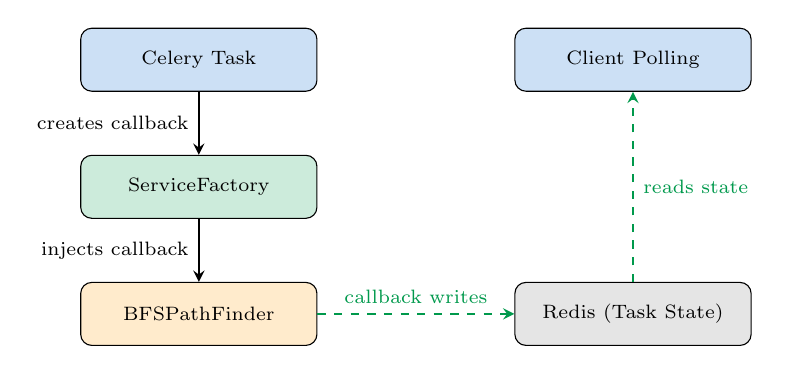
\begin{tikzpicture}[
    node distance=0.8cm,
    box/.style={draw, rounded corners, minimum width=3cm, minimum height=0.8cm, align=center, font=\scriptsize},
    arrow/.style={->, thick, >=stealth},
    darrow/.style={->, thick, >=stealth, dashed, color=accentgreen}
]
    \node[box, fill=accentblue!20] (task) {Celery Task};
    \node[box, fill=accentgreen!20, below=of task] (factory) {ServiceFactory};
    \node[box, fill=warningorange!20, below=of factory] (pathfinder) {BFSPathFinder};
    \node[box, fill=codegray!20, right=2.5cm of pathfinder] (redis) {Redis (Task State)};
    \node[box, fill=accentblue!20, right=2.5cm of task] (client) {Client Polling};
    
    \draw[arrow] (task) -- node[left, font=\scriptsize] {creates callback} (factory);
    \draw[arrow] (factory) -- node[left, font=\scriptsize] {injects callback} (pathfinder);
    \draw[darrow] (pathfinder) -- node[above, font=\scriptsize] {callback writes} (redis);
    \draw[darrow] (redis) -- node[right, font=\scriptsize] {reads state} (client);
\end{tikzpicture}
\end{center}

\subsection{Why This Design?}

\begin{tabularx}{\textwidth}{@{}>{\bfseries}l X@{}}
\toprule
Benefit & Explanation \\
\midrule
Decoupling & The BFS algorithm doesn't know about Celery. It just calls a function. \\
\addlinespace[0.3em]
Testability & In tests, pass a mock callback that records calls instead of updating Celery. \\
\addlinespace[0.3em]
Flexibility & Easy to change reporting frequency or add more metrics without touching BFS. \\
\addlinespace[0.3em]
No Polling Inside Worker & Worker doesn't poll; it pushes. Client pulls on its own schedule. \\
\bottomrule
\end{tabularx}

% ============================================
% SECTION 6: DEPENDENCY INJECTION
% ============================================
\section{Dependency Injection (DI) Explained}

\begin{notebox}
\textbf{Location:} \texttt{app/core/factory.py} -- \texttt{ServiceFactory} class
\end{notebox}

\subsection{The Pattern: Singleton + Factory}

\begin{lstlisting}[caption=ServiceFactory Implementation]
class ServiceFactory:
    _redis_client = None      # Singleton storage
    _cache_service = None
    _wikipedia_client = None
    
    @classmethod
    def get_cache_service(cls):
        if cls._cache_service is None:
            redis_client = cls.get_redis_client()
            cls._cache_service = RedisCache(redis_client)
        return cls._cache_service
    
    @classmethod
    def create_pathfinding_service(cls, algorithm="bfs", progress_callback=None):
        # Retrieve singletons, then inject into new instance
        wiki = cls.get_wikipedia_client()
        cache = cls.get_cache_service()
        queue = cls.get_queue_service()
        
        path_finder = RedisBasedBFSPathFinder(wiki, cache, queue, progress_callback)
        return PathFindingService(path_finder, cache, wiki)
\end{lstlisting}

\subsection{Swapping Implementations}

To use Memcached instead of Redis:
\begin{enumerate}[leftmargin=*, nosep]
    \item Create \texttt{MemcachedCache} implementing \texttt{CacheServiceInterface}.
    \item Modify \texttt{ServiceFactory.get\_cache\_service()} to return \texttt{MemcachedCache}.
    \item Done. All services automatically use the new cache.
\end{enumerate}

% ============================================
% SECTION 7: FILE BY FILE BREAKDOWN
% ============================================
\section{File-by-File Breakdown}

\subsection{Core Files}

\begin{tabularx}{\textwidth}{@{}>{\ttfamily}l X@{}}
\toprule
\normalfont\textbf{File} & \textbf{Purpose} \\
\midrule
app/core/pathfinding.py & \textbf{CORE ALGORITHM}. Redis-based BFS. Modify for algorithm changes. \\
\addlinespace[0.3em]
app/core/services.py & Business orchestration. Cache checking, validation, timing. \\
\addlinespace[0.3em]
app/core/factory.py & DI container. Manages singletons and object creation. \\
\addlinespace[0.3em]
app/core/interfaces.py & Abstract contracts for testability and loose coupling. \\
\addlinespace[0.3em]
app/core/models.py & Dataclasses for requests, results, and DTOs. \\
\bottomrule
\end{tabularx}

\subsection{Infrastructure Files}

\begin{tabularx}{\textwidth}{@{}>{\ttfamily}l X@{}}
\toprule
\normalfont\textbf{File} & \textbf{Purpose} \\
\midrule
app/infrastructure/cache.py & Redis cache implementation with connection pooling. \\
\addlinespace[0.3em]
app/infrastructure/redis\_queue.py & FIFO queue for BFS state (push, pop, length). \\
\addlinespace[0.3em]
app/infrastructure/tasks.py & Celery task definitions with retry logic and progress updates. \\
\addlinespace[0.3em]
app/external/wikipedia.py & Wikipedia API client with bulk fetching and redirect handling. \\
\bottomrule
\end{tabularx}

% ============================================
% SECTION 8: CACHING STRATEGY
% ============================================
\section{Caching Strategy}

\begin{tabularx}{\textwidth}{@{}>{\ttfamily}l l X@{}}
\toprule
\normalfont\textbf{Key Pattern} & \textbf{TTL} & \textbf{Purpose} \\
\midrule
wiki\_links:\{page\} & 24h & Caches Wikipedia page links. High reuse. \\
path:\{start\}:\{end\} & 1h & Caches completed path results. \\
bfs\_visited:<uuid>:* & 1h & Temporary visited set. Cleaned after search. \\
bfs\_paths:<uuid>:* & 1h & Temporary path tracking. Cleaned after search. \\
bfs\_queue:<uuid> & Session & BFS queue. Explicitly deleted after search. \\
\bottomrule
\end{tabularx}

% ============================================
% SECTION 9: INTERVIEW Q&A CHEAT SHEET
% ============================================
\section{Interview Q\&A Cheat Sheet}

\begin{qabox}{If you had to modify the core pathfinding algorithm, where would you go?}
\textbf{Answer:} \texttt{app/core/pathfinding.py} -- specifically the \texttt{RedisBasedBFSPathFinder} class and its \texttt{find\_shortest\_path()} method.
\end{qabox}

\begin{qabox}{When and where do services get initialized?}
\textbf{Answer:} Services are \textbf{lazily initialized} by \texttt{ServiceFactory} (\texttt{app/core/factory.py}) on first use. Not at app startup. Flask: first request. Celery: first task.
\end{qabox}

\begin{qabox}{Which objects are reused vs. created fresh?}
\textbf{Answer:}
\begin{itemize}[leftmargin=*, nosep]
    \item \textbf{Reused (Singletons):} Redis Client, Wikipedia Client, Cache Service. Maintains connection pools.
    \item \textbf{Fresh (Transient):} PathFindingService. New per task for isolated callbacks.
\end{itemize}
\end{qabox}

\begin{qabox}{How does the progress callback work?}
\textbf{Answer:} 
\begin{enumerate}[leftmargin=*, nosep]
    \item Celery task defines a closure that calls \texttt{self.update\_state()}.
    \item This closure is passed to \texttt{ServiceFactory.create\_pathfinding\_service()}.
    \item Factory injects it into \texttt{RedisBasedBFSPathFinder} constructor.
    \item BFS calls the callback every N nodes, writing progress to Redis.
    \item Client polls \texttt{/tasks/status/<id>} to read progress.
\end{enumerate}
\end{qabox}

\begin{qabox}{Why use Celery instead of handling pathfinding synchronously?}
\textbf{Answer:} Pathfinding can take minutes. Synchronous handling would:
\begin{itemize}[leftmargin=*, nosep]
    \item Timeout HTTP connections (typically 30-60s limit).
    \item Block web server threads, reducing throughput.
    \item Provide no progress visibility to users.
\end{itemize}
Celery enables horizontal scaling, resilience, and real-time progress.
\end{qabox}

\begin{qabox}{Why Redis for BFS queue instead of Python deque?}
\textbf{Answer:} Memory safety. BFS at depth 5+ can involve millions of nodes. Redis:
\begin{itemize}[leftmargin=*, nosep]
    \item Offloads memory from worker process.
    \item Enables inspection via Redis CLI.
    \item Provides crash-recovery potential (state persists).
\end{itemize}
Trade-off: Network latency per operation (mitigated by batching).
\end{qabox}

\begin{qabox}{How does the system scale horizontally?}
\textbf{Answer:}
\begin{itemize}[leftmargin=*, nosep]
    \item \textbf{API:} Stateless Flask servers behind load balancer.
    \item \textbf{Workers:} Add Celery workers to increase search throughput.
    \item \textbf{Cache:} Redis Cluster for sharding and replication.
\end{itemize}
\end{qabox}

\begin{qabox}{Explain singletons across processes.}
\textbf{Answer:} Singletons are per-process. 4 Gunicorn workers = 4 Wikipedia Clients. They share state via Redis (the database is the shared memory), not in-process memory.
\end{qabox}

\begin{qabox}{Why is the Wikipedia Client a singleton?}
\textbf{Answer:} It holds a \texttt{requests.Session} which provides:
\begin{itemize}[leftmargin=*, nosep]
    \item HTTP Keep-Alive (connection reuse).
    \item TLS session resumption (avoids 100-300ms handshake).
    \item Cookie persistence if needed.
\end{itemize}
Creating new clients per request would destroy these benefits.
\end{qabox}

\begin{qabox}{How would you add a new pathfinding algorithm?}
\textbf{Answer:}
\begin{enumerate}[leftmargin=*, nosep]
    \item Create class implementing \texttt{PathFinderInterface} in \texttt{pathfinding.py}.
    \item Add case in \texttt{ServiceFactory.create\_pathfinding\_service()}.
    \item Update API schema to accept new algorithm name.
    \item Add tests in \texttt{tests/integration/test\_pathfinding.py}.
\end{enumerate}
\end{qabox}

% ============================================
% SECTION 10: QUICK REFERENCE
% ============================================
\section{Quick Reference: Where to Make Changes}

\begin{tabularx}{\textwidth}{@{}>{\bfseries}l X@{}}
\toprule
Goal & Location \\
\midrule
Modify BFS algorithm & \texttt{app/core/pathfinding.py} \\
Add new API endpoint & \texttt{app/api/routes.py} \\
Change request validation & \texttt{app/api/schemas.py} \\
Add new Celery task & \texttt{app/infrastructure/tasks.py} \\
Swap cache implementation & Implement interface, update \texttt{factory.py} \\
Add new exception type & \texttt{app/utils/exceptions.py} \\
Change configuration & \texttt{config/base.py} \\
Modify Wikipedia API logic & \texttt{app/external/wikipedia.py} \\
\bottomrule
\end{tabularx}

% ============================================
% SECTION 11: API ENDPOINTS
% ============================================
\section{API Endpoints Reference}

\begin{tabularx}{\textwidth}{@{}l >{\ttfamily}l X@{}}
\toprule
\textbf{Method} & \normalfont\textbf{Endpoint} & \textbf{Description} \\
\midrule
POST & /getPath & Start pathfinding. Returns task ID. \\
GET & /tasks/status/<id> & Poll for task status and progress. \\
POST & /explore & Explore links from a page. \\
GET & /health & System health check. \\
GET & /api & API information. \\
POST & /cache/clear & Admin: clear cache by pattern. \\
\bottomrule
\end{tabularx}

% ============================================
% SECTION 12: CONFIGURATION
% ============================================
\section{Configuration Reference}

\begin{tabularx}{\textwidth}{@{}>{\ttfamily}l l X@{}}
\toprule
\normalfont\textbf{Variable} & \textbf{Default} & \textbf{Description} \\
\midrule
REDIS\_URL & localhost:6379 & Redis connection URL. \\
MAX\_SEARCH\_DEPTH & 6 & Maximum BFS depth. \\
BFS\_BATCH\_SIZE & 50 & Pages per batch in BFS. \\
CACHE\_TTL & 86400 & Default cache TTL (24h). \\
WIKIPEDIA\_MAX\_WORKERS & 10 & Thread pool for Wikipedia API. \\
CELERY\_TASK\_SOFT\_TIME\_LIMIT & 300 & Soft timeout (5m). \\
CELERY\_TASK\_TIME\_LIMIT & 600 & Hard timeout (10m). \\
\bottomrule
\end{tabularx}

% ============================================
% END
% ============================================

\end{document}
